\subsection{State (\textit{o Object for States})}
\label{state}

\textbf{Scopo}: Comportamentale \\
\textbf{Raggio d'azione}: Oggetti

\paragraph{Definizione} Il pattern State consente ad un oggetto di modificare il proprio comportamento quando cambia il suo stato interno. L'oggetto \textit{sembrerà} cambiare classe.

\paragraph{Motivazione} Considera una classe TCPConnection che rappresenta una connessione di rete, dove un oggetto TCPConnection può essere in uno di diversi stati: Established, Listening, Closed. Quando un oggetto TCPConnection riceve richieste da altri oggetti, risponde diversamente a seconda del suo stato corrente: per esempio, l'effetto di una richiesta Open dipende dal fatto che la connessione sia nel suo stato Closed o nel suo stato Established. 

\begin{figure}[H]
    \centering
    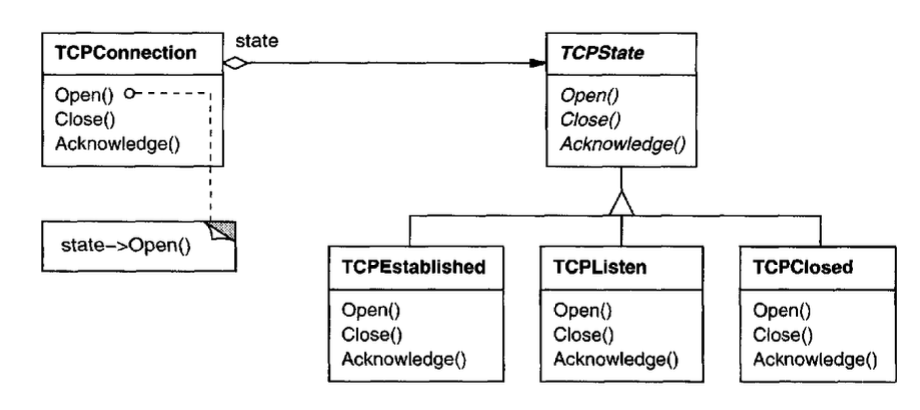
\includegraphics[width=0.75\linewidth]{assets/pattern/state/state-esempio.png}
\end{figure}

Il pattern State descrive come TCPConnection possa esibire comportamenti diversi in ogni stato, e l'idea chiave in questo pattern è introdurre una classe astratta chiamata TCPState per rappresentare gli stati della connessione di rete, dove la classe TCPState dichiara un'interfaccia comune a tutte le classi che rappresentano stati operazionali diversi, e le sottoclassi di TCPState implementano comportamento specifico dello stato, per esempio le classi TCPEstablished e TCPClosed implementano comportamento particolare agli stati Established e Closed di TCPConnection. La classe TCPConnection mantiene un oggetto stato (un'istanza di una sottoclasse di TCPState) che rappresenta lo stato corrente della connessione TCP, e TCPConnection delega tutte le richieste specifiche dello stato a questo oggetto stato, usando la sua istanza di sottoclasse TCPState per eseguire operazioni particolari allo stato della connessione. Ogni volta che la connessione cambia stato, l'oggetto TCPConnection cambia l'oggetto stato che usa: quando la connessione va da established a closed, per esempio, TCPConnection sostituirà la sua istanza TCPEstablished con un'istanza TCPClosed.

\paragraph{Applicabilità} È opportuno usare il pattern State quando:
\begin{itemize}
    \item Il comportamento di un oggetto dipende dal suo stato e deve cambiare in fase di esecuzione a seconda di esso.
    \item Le operazioni hanno istruzioni condizionali grandi e multiparte che dipendono dallo stato dell'oggetto: questo stato è solitamente rappresentato da una o più costanti enumerate.
    \item Diverse operazioni contengono la stessa struttura condizionale: il modello State inserisce ogni ramo condizionale in una classe separata (per evitare di applicazioni azioni diverse con comandi quali switch). Ciò consente di trattare lo stato dell'oggetto come un oggetto a sé stante che può variare indipendentemente dagli altri oggetti.
\end{itemize}

\begin{figure}[H]
    \centering
    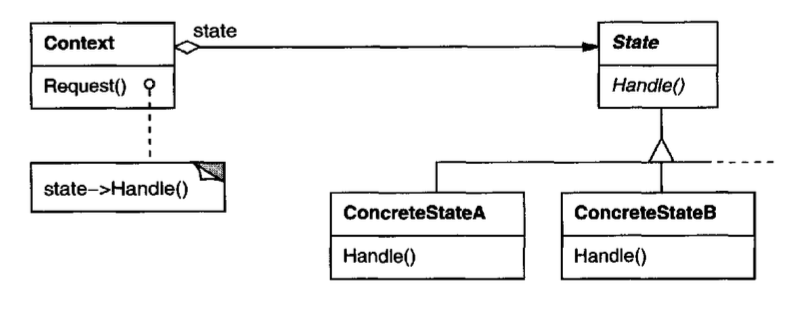
\includegraphics[width=0.75\linewidth]{assets/pattern/state/state-struttura.png}
    \caption{Class Diagram del pattern}
\end{figure}

\paragraph{Struttura} Il pattern è composto da:
\begin{itemize}
    \item \textbf{Context}: definisce l’interfaccia utilizzata dai client. Mantiene un riferimento ad un’istanza di una classe che implementa l’interfaccia State e che rappresenta lo stato corrente.
    \item \textbf{State}: Definisce un’interfaccia che incapsula il comportamento associato ad uno stato particolare di Context.
    \item \textbf{ConcreteState}: Ogni classe che occupa questo ruolo definisce un particolare comportamento associato ad uno stato di Context.
\end{itemize}

\paragraph{Conseguenze} Il pattern State consente quindi di:
\begin{itemize}
    \item Localizzare il comportamento specifico dello stato e suddividere il comportamento per stati diversi.
    \item Rendere esplicite le transizioni di stato (atomiche dal p.d.v. di Context)
    \item Condividere gli oggetti State
\end{itemize}

È bene notare che l'applicazione del modello risulta eccessiva per applicazioni che presentano pochi stati o che cambiano raramente.

\paragraph{Pattern correlati} Può essere correlato ai pattern Flyweight (\ref{flyweight}, utilizzato per la condivisione di oggetti State) e Singleton (\ref{singleton}, spesso gli oggetti State sono dei Singleton)

\newpage